% \documentclass[aspectratio=169]{beamer}
\documentclass{beamer}
\usepackage[utf8]{inputenc}
\usepackage[document]{ragged2e}
\usepackage{tiks}
\usetheme{Colmeia}

% Título
\title{\textbf{Template padrão para Aprensentações em \LaTeX}}

% Autor(es), separar por \&
\author{Paulo Henrique Cuchi \& Daniel S. Camargo}

\institute[UDESC]{
    % Logo do COLMEIA
    
\includegraphics[height=1.3cm]{images/colmeia.png}\\[1em]
    Universidade do Estado de Santa Catarina
}

\date{
    % Data
    25 de Abril de 2015\\[1em]

    % ############################# IMPORTANTE ################################
    % Selo da licença. Nesse caso é domínio público (cc0), porém, quando
    % divulgar seu trabalho, coloque Creative Commons - Atribuição (ccby.png)
    %
\includegraphics[width=1.3cm]{ccby.png}\\[1em]
    
\includegraphics[width=1.3cm]{images/cc0.png}
    %
\includegraphics[width=1.3cm]{images/ccby.png}
}

%%%%%%%%%%%%%%%%%%%%%%%%%%%%%%%%%%%%%%%%%%%%%%%%%%%%%%%%%%%%%%%%%%%%%%%%%%%%%%%
%%%%%%%%%%%%%%%%%%%%%%%%%%%%%%%%%%%%%%%%%%%%%%%%%%%%%%%%%%%%%%%%%%%%%%%%%%%%%%%
%%%%%%%%%%%%%%%%%%%%%%%%%%%%%%%%%%%%%%%%%%%%%%%%%%%%%%%%%%%%%%%%%%%%%%%%%%%%%%%

\begin{document}
% Remove os ícones de navegação:
\beamertemplatenavigationsymbolsempty

\frame{\titlepage}

% Marca d'água
\usebackgroundtemplate{
    \tikz[overlay, remember picture]
    \node[at=(current page.south east),anchor=south east,inner sep=0pt] {
        
\includegraphics[height=\paperheight]{images/background.png}
    };
}

% Sumário
\frame{\tableofcontents}

%%%%%%%%%%%%%%%%%%%%%%%%%%%%%%%%%%%%%%%%%%%%%%%%%%%%%%%%%%%%%%%%%%%%%%%%%%%%%%%
% O ConteÚdo começa aqui %%%%%%%%%%%%%%%%%%%%%%%%%%%%%%%%%%%%%%%%%%%%%%%%%%%%%%
%%%%%%%%%%%%%%%%%%%%%%%%%%%%%%%%%%%%%%%%%%%%%%%%%%%%%%%%%%%%%%%%%%%%%%%%%%%%%%%

\section{Hello World!}
\frame{
    \frametitle{Hello World!}
    Esse é o template oficial do COLMEIA para a criação de apresentações no
    Beamer - \LaTeX.\\[1em]
    Abra o código-fonte (arquivo \textit{beamer.tex}) para começar a editar.
    Qualquer um que não tenha utilizado Beamer pode aprender facilmente com os
    comentáros e exemplos prontos no código.\\[1em]
    Para ``compilar'' o arquivo .tex, utilize o comando \textit{pdflatex}. É
    recomendado que repita o comando 3 vezes para resolver referências
    cruzadas.
}

\subsection{Texto}
\frame{
    Esse slide faz parte da subseção ``Texto'', ele não possui o titulo, que é
    opcional.
}

\frame{
    \frametitle{Texto}
    É recomendado que o número de subseções não ultrapasse de 3, para que não
    distorça o cabeçalho.\\[1em]
    Use \textbf{negrito} e \textit{itálico} quando achar necessário, e não
    esqueça de separar os tópicos por parágrafos. Em geral, evite textos
    longos, isso evita que sua apresentação fique cansativa.\\[1em]\pause
    O texto pode conter pausas, \pause o que pode ajudar a organizar os
    tópicos por ordem de explicação, \pause sem dar spoilers.
}

\frame{
    \frametitle{Texto}
    Use colunas para encaixar uma imagem junto ao texto. o \textit{justify} pode ajudar
    na estética.
    \begin{columns}
        \begin{column}{0.6\textwidth}
            \justify
            \begin{small}
                ``O núcleo Linux foi, originalmente, escrito por Linus Torvalds do
                Departamento de Ciência da Computação da Universidade de Helsinki,
                Finlândia, com a ajuda de vários programadores voluntários através
                da Usenet (uma espécie de sistema de listas de discussão existente
                desde os primórdios da Internet).'' Wikipedia
            \end{small}
        \end{column}
        \begin{column}{0.4\textwidth}
            
\includegraphics[width=\textwidth]{images/tux.png}
        \end{column}
    \end{columns}
}

\frame{
    \frametitle{Texto}
    O texto pode ter diversos tamanhos, os mais relevantes são:\\[1em]
    \begin{center}
        \tiny{Tiny}\\
        \small{Small}\\
        \LARGE{Large}\\
        \Huge{Huge}
    \end{center}
}

\frame{
    \begin{center}
    \Large{Seja \textcolor{blue}{\textbf{criativo}} quando for enfatizar algo.}
    \end{center}
}

\section{Listas}
\frame{
    \frametitle{Listas}
    Listas são fáceis de fazer, sejam elas não numeradas:
    \begin{itemize}
        \item{C++}
        \item{Python}
        \item{Haskell}
        \item{Ruby}
    \end{itemize}
}

\frame{
    \frametitle{Listas}
    ...ou numeradas:
    \begin{enumerate}
        \item{C++}
        \item{Python}
        \item{Haskell}
        \item{Ruby}
    \end{enumerate}
}

\frame{
    \frametitle{Listas}
    Pausas também podem ser usadas em listas:\pause
    \begin{itemize}
        \item{C++\pause}
        \item{Python\pause}
        \item{Haskell\pause}
        \item{Ruby}
    \end{itemize}
}

\section{Tabelas e Imagens}

\frame{
    \frametitle{Tabelas e Imagens}
    Tabelas e imagens ficam melhores quando são centralizadas.
}

\subsection{Tabelas}
\frame{
    \frametitle{Tabelas}
    \begin{center}
        \begin{tabular}{|c|c|c|}
            \hline
            \textbf{Sigla} & \textbf{Matéria} & \textbf{Nota} \\
            \hline
            CDI2 & Cálculo Diferencial e Integral 2 & 1.3 \\
            \hline
            ALG2 & Algebra Linear 2 & 0.5 \\
            \hline
            SOP & Sistemas Operacionais & 9.8 \\
            \hline
            CAL & Complexidade de Algorítimos & 8.6 \\
            \hline
        \end{tabular}
    \end{center}
}

\subsection{Imagens}
\frame{
    \frametitle{Imagens}
    \begin{center}
        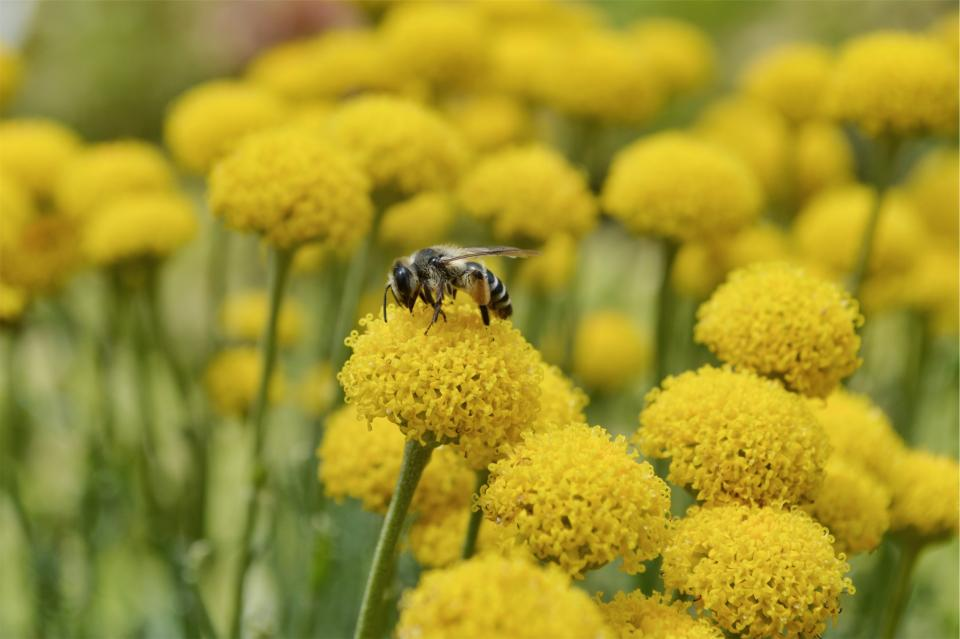
\includegraphics[width=0.5\textwidth]{images/bee.jpg}
    \end{center}
}

\section{Blocos}
\frame{
    \frametitle{Blocos}
    Blocos podem ser usados para observações e exemplos.
    \begin{block}{Bloco comum}
        block
    \end{block}

    \begin{exampleblock}{Bloco para exemplificar algo}
        exampleblock
    \end{exampleblock}

    \begin{alertblock}{Bloco de alerta}
        alertblock
    \end{alertblock}
    A única diferença é a cor.
}

\section{Material Complementar}
\frame{
    \frametitle{Material Complementar}
    Clique nos items para abrir:
    \begin{itemize}
        \item{\href{http://www.academia.edu/4975170/Apostila\_de\_LaTeX\_Criando\_Artigos\_Acadêmicos}{Apostila de LaTeX - Daniel S. Camargo}}
        \item{\href{http://http://tex.stackexchange.com/}{LaTeX Stack Exchange}}
    \end{itemize}
}

\section{Contato}
\frame{
    \textbf{Dúvidas? entre em contato!}\\[1em]
    \begin{center}
        paulo.cuchi@colmeia.udesc.br\\
        daniel@colmeia.udesc.br
    \end{center}
}
\end{document}
